\documentclass[]{article}
\usepackage{float,graphicx}
\usepackage{tikz}


\title{test}

\begin{document}
    \section{lines}
    % [xscale=2.5, yscale=0.5]
    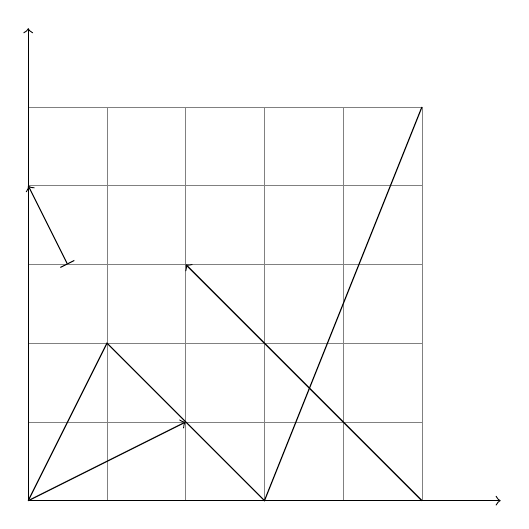
\begin{tikzpicture}[scale=1]
        \draw[help lines] (0,0) grid(5,5);
        \draw (0,0) -- (1,2)--(3,0) --(5,5);
        
        \draw [->] (0,0) -- (2,1);
        
        \draw [<-] (2,3) -- (5,0);
        
        \draw [|->] (0.5,3) -- (0,4);
        
        \draw [<->] (0,6) -- (0,0) -- (6,0);
        
    \end{tikzpicture}
    
    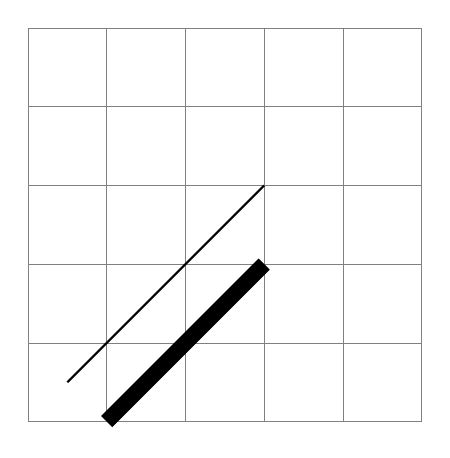
\begin{tikzpicture}
        \draw[help lines] (0,0) grid(5,5);
        \draw[thick] (0.5, 0.5) -- (3,3);
        % [ultra thick, thick, thin, very thick]
        \draw[line width=0.2cm] (1,0) -- (3,2);
    \end{tikzpicture}
    
    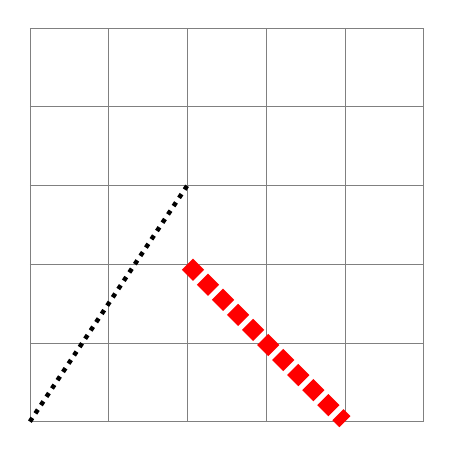
\begin{tikzpicture}
        \draw[help lines] (0,0) grid(5,5);
        \draw[ultra thick, dotted] (0,0) -- (2,3);
        \draw[line width=0.2cm, dotted,red] (2,2) -- (4,0);
        
        %[red, blue, green, cyan, magenta, yellow, black, gray, darkgray, lightgray, browbn, lime, olive, orange, pink, purple, teal, violet, white]
    \end{tikzpicture}
    \newpage
    \section{curves}
    
    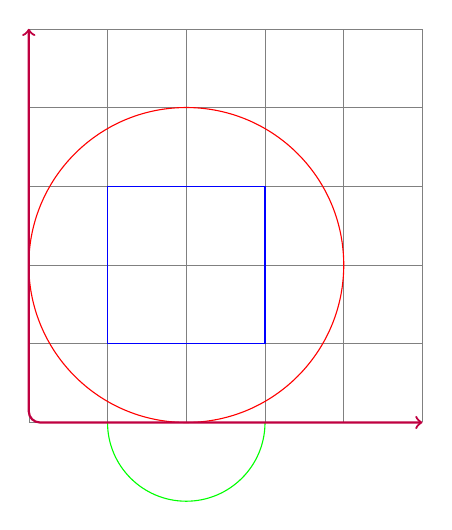
\begin{tikzpicture}
        \draw[help lines] (0,0) grid(5,5);
        \draw[blue] (1,1) rectangle(3,3);
        \draw[red] (2,2) circle[radius=2];
        \draw[green] (1,0) arc [radius=1,start angle=180,end angle=360];
        
        \draw[<->, rounded corners, thick, purple] (0,5) -- (0,0) -- (5,0);
    
    \end{tikzpicture}

    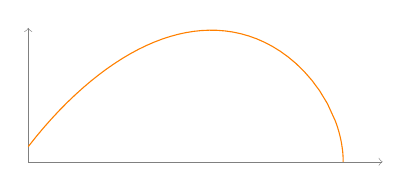
\begin{tikzpicture}[xscale=10,yscale=5]
    \draw [<->, help lines] (0.6,1.34) -- (0.6,1) -- (1.05,1);
    \draw[orange] (0.6, 1.0385) --
(0.61, 1.06372) -- (0.62, 1.08756) -- (0.63, 1.11012) -- (0.64,
1.13147) -- (0.65, 1.15166) -- (0.66, 1.17074) -- (0.67, 1.18874) -- (0.68,
1.20568) -- (0.69, 1.22157) -- (0.7, 1.23643) -- (0.71, 1.25026) -- (0.72,
1.26307) -- (0.73, 1.27486) -- (0.74, 1.28561) -- (0.75, 1.29534) -- (0.76,
1.30402) -- (0.77, 1.31165) -- (0.78, 1.31821) -- (0.79, 1.32369) -- (0.8,
1.32806) -- (0.81, 1.33131) -- (0.82, 1.3334) -- (0.83, 1.33431) -- (0.84,
1.334) -- (0.85, 1.33244) -- (0.86, 1.32956) -- (0.87, 1.32533) -- (0.88,
1.31966) -- (0.89, 1.3125) -- (0.9, 1.30373) -- (0.91, 1.29325) -- (0.92,
1.2809) -- (0.93, 1.26649) -- (0.94, 1.24976) -- (0.95, 1.23032) -- (0.96,
1.2076) -- (0.97, 1.18065) -- (0.98, 1.14763) -- (0.99, 1.1038) -- (0.991,
1.09836) -- (0.992, 1.09261) -- (0.993, 1.0865) -- (0.994, 1.07994) -- (0.995,
1.07282) -- (0.996, 1.06497) -- (0.997, 1.0561) -- (0.998, 1.04563) -- (0.999,
1.03209) -- (0.9991, 1.03042) -- (0.9992, 1.02866) -- (0.9993,
1.02679) -- (0.9994, 1.02478) -- (0.9995, 1.0226) -- (0.9996, 1.02019) -- (0.9997,
1.01747) -- (0.9998, 1.01424) -- (0.9999, 1.01005) -- (0.9999,
1.01005) -- (0.99991, 1.00953) -- (0.99992, 1.00898) -- (0.99993,
1.0084) -- (0.99994, 1.00778) -- (0.99995, 1.0071) -- (0.99996,
1.00634) -- (0.99997, 1.00549) -- (0.99998, 1.00448) -- (0.99999, 1.00317) -- (1,
1) ;
        
    
    \end{tikzpicture}
    
    This gives us a curve from (0,0) to (2,1.5) which leaves at an angle of 90◦ and
arrive at an angle of 195◦

    \begin{tikzpicture}
    \draw[help lines] (0,0) grid(2,2);
        \draw[ultra thick](0,0) to [out=90,int=195] (2,1.5);
    \end{tikzpicture}
    
    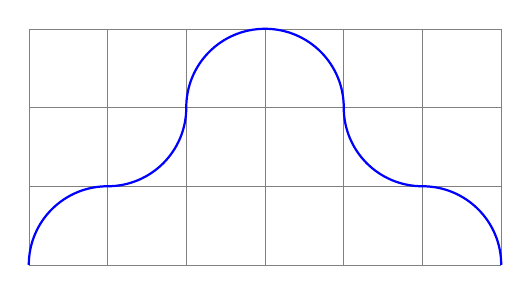
\begin{tikzpicture}
        \draw[help lines] (0,0) grid(6,3);
        \draw[blue, thick] (0,0) to[out=90,in=180] (1,1) to[in=270,out=360] (2,2)
        to[in=180,out=90] (3,3) to[in=90,out=360] (4,2) to[in=180,out=270] (5,1) 
        to[in=90, out=0] (6,0);
    \end{tikzpicture}
    
    \section{plotting functions}
        
    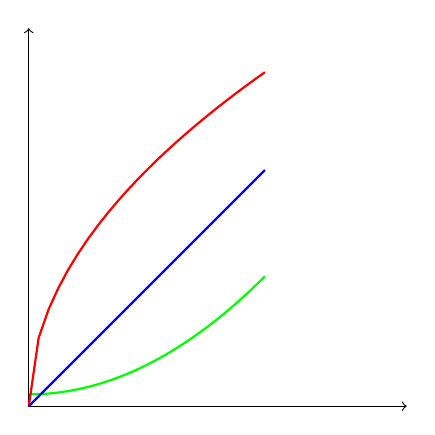
\begin{tikzpicture}[xscale=6,yscale=6]
        
        \draw[<->] (0,0.8) -- (0,0) -- (0.8,0);
        \draw[green,thick,domain=0:0.5]
        plot(\x, {0.025+\x*\x});
        
        \draw[red, thick, domain=0:0.5]
        plot(\x, {sqrt(\x)});
        
        \draw[blue, thick, domain=0:0.5]
        plot(\x, {abs(\x)});
        
    \end{tikzpicture}
    
    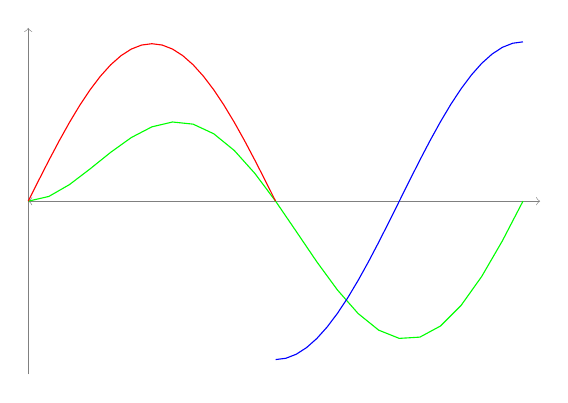
\begin{tikzpicture}[yscale=2]
    \draw [help lines, <->] (0,0) -- (6.5,0);
    \draw [help lines, ->] (0,-1.1) -- (0,1.1); 
        \draw [green,domain=0:2*pi] plot (\x, {(sin(\x r)* ln(\x+1))/2});
        \draw [red,domain=0:pi] plot (\x, {sin(\x r)});
        \draw [blue, domain=pi:2*pi] plot (\x, {cos(\x r)*exp(\x/exp(2*pi))});

    \end{tikzpicture}
    
    \section{Filling up areas}

        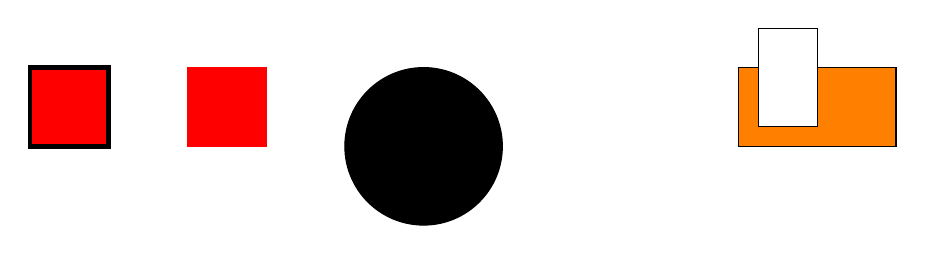
\begin{tikzpicture}
            \draw[fill=red,ultra thick] (0,0) rectangle(1,1);
            
            \draw[fill=red,ultra thin, red] (2,0) rectangle(3,1);
            
            \draw[fill] (5,0) circle[radius=1];
            
            \draw [fill=orange] (9,0) rectangle (11,1);
            \draw [fill=white] (9.25,0.25) rectangle (10,1.5);
            
        \end{tikzpicture}
        
        
    
\begin{tikzpicture}
        \path [fill=gray] (0,0) rectangle (1.5,1);
        \draw [fill=yellow] (2,0) rectangle (3.5,1);
    \end{tikzpicture}
    
    
    \section{putting labels in pictures}
    
    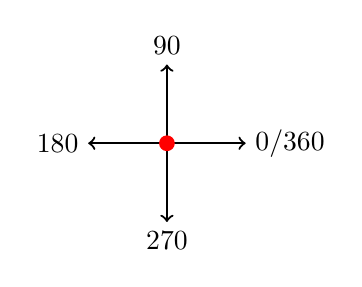
\begin{tikzpicture}
        \draw[<->,black, thick] (0,-1) -- (0,1);
        \draw[<->,black, thick] (1, 0) -- (-1,0);
        \path[thick, fill=red] (0,0) circle[radius=0.1];
        
        \node[right] at (1,0) {0/360};
        \node[above] at (0, 1) {90};
        \node[left] at (-1, 0) {180};
        \node[below] at (0,-1) {270};
    \end{tikzpicture}
    
    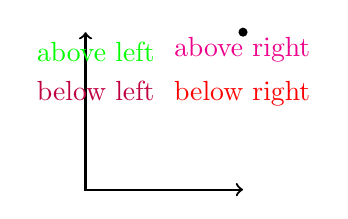
\begin{tikzpicture}[scale=2]
        \draw [thick, <->] (0,1) -- (0,0) -- (1,0);
        \draw[fill] (1,1) circle [radius=0.025];
        \node [below right, red] at (.5,.75) {below right};
        \node [above left, green] at (.5,.75) {above left};
        \node [below left, purple] at (.5,.75) {below left};
        \node [above right, magenta] at (.5,.75) {above right};
    \end{tikzpicture}
    
    \begin{tikzpicture}[scale=2]
        \draw[<->, thick] (0,1) -- (0,0) -- (1,0);
        \node[above left, black, thick] at (0,1) {$y$};
        \node[below right, black, thick] at (1,0) {$x$};
        \draw[fill=black] (0.5,0.5) circle[radius=0.5pt];
        \draw[red] (0.5,0.5) circle[radius=0.1];

        \node[above right] at (0.5,0.5) {$A$};
    \end{tikzpicture}

    \begin{tikzpicture}[xscale=3, yscale=3]
    \draw [thick, <->] (0,1) node [left] {$y$}
    -- (0,0) -- (1,0) node [below right] {$x$};
    \draw[fill] (.4,.6) circle [radius=.5pt]
    node[above right] (.4,.6) {$A$};
    \end{tikzpicture}
    
    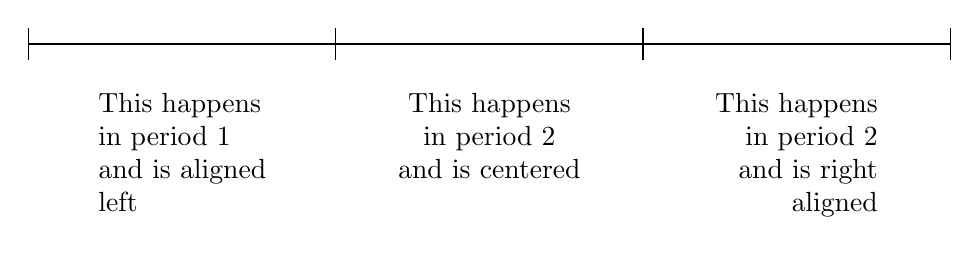
\begin{tikzpicture}[xscale=1.3]
    \draw [thick] (0,0) -- (9,0);
    \draw (0,-.2) -- (0, .2);
    \draw (3,-.2) -- (3, .2);
    \draw (6,-.2) -- (6, .2);
    \draw (9,-.2) -- (9, .2);
    \node[align=left, below] at (1.5,-.5)%
    {This happens\\in period 1\\and is aligned\\ left};
    \node[align=center, below] at (4.5,-.5)%
    {This happens\\in period 2\\and is centered};
    \node[align=right, below] at (7.5,-.5)%
    {This happens\\in period 2\\and is right\\aligned};
    \end{tikzpicture}
    
    \begin{tikzpicture}
        \draw[help lines] (0,0) grid(3,3);
        \draw[thick] (0,0,0) -- (0,0,3); 
        \draw[thick] (0,0,0) -- (0,3,0);
        \draw[thick] (0,0,0) -- (3,0,0);
    \end{tikzpicture}

\end{document}